\externaldocument{../3/chapter_modeling}
\externaldocument{../4/chapter_algorithm}
\startchapter{Dual\_trace Communication Analysis Prototype In Atlantis}
\label{chapter:newsol}
In this chapter, I present the design of the prototype of communication analysis from the dual\_trace. This prototype is implemented in Atlantis. Atlantis is an assembly-level execution trace analysis environment. It provides many features that benefit the communication analysis of dual\_trace. 

This prototype consists of four components: 1) declaring the functions descriptors of the communication methods, 2) a view that can display both traces in the dual\_trace in parallel, 3) implementation of the communication analysis algorithms for stream extraction and communication identification, and 4) a view for presenting the extracted streams and the identified communications from the dual\_trace.

\section{Use Cases}
In this section, two use cases are presented to depict how to use the developed components and the existing features of Atlantis to perform the communication analysis.

To analyze a dual\_trace, the user needs to perform the below operations in sequence:
\begin{itemize}
\item Open two traces in a parallel view (as part of this prototype)
\item Import the dynamic-linked library files for each trace (as part of the existing functionality of Atlantis)
\item Perform the stream extraction or communication identification operations (as part of this prototype)
\item Inspect the operation results by navigating the analysis results from the communication view (as part of this prototype).
\end{itemize}

Two use cases of this prototype are designed. The use case shown in Table \ref{usecase1} is for stream extraction. The goal of this use case is to analyze two execution traces in a dual\_trace and output the streams of each trace. The use case shown in Table \ref{usecase2} is for identifying the concerned communication from a dual\_trace. 

\begin{table}[H]
  \centering
  \caption{Use case 1: extract streams from a dual\_trace}
  \label{usecase1}
  \begin{tabular}{|l|p{13cm}|}
      \hline
       \textbf{Name} & Analysis streams of a communication method from the Dual\_trace\\
       \hline
       \textbf{Description} & A user capture two assembly-level execution traces of two interacting programs and needs to analysis them by extracting all communication streams of each of the traces and inspecting the extraction results \\
       \hline
              \textbf{Actor} & A software security engineer \\
       \hline
       \textbf{Precondition} & The user has two assembly-level execution traces and the .dll files of the systems where the programs of the captured traces were running\\
       \hline
       \textbf{Main Course}& 1. The user declares the functions descriptors for the communication methods of interest in a Json format setting file\\
        & 2. The user opens one of the trace in Atlantis\\
       &  3. The user opens the other trace as the dual\_trace of the first one\\
       & 4. The two opened traces are presented in the parallel view\\
       & 5. The user loads the related .dll files for both opened traces\\
       & 6. The user selects the operation ``Stream Extraction" in the ``Dual\_Trace Tool" menu.\\
       & 7. Atlantis prompts a dialog window giving the user all the communication methods in the functions descriptor setting file as options\\
       & 8. The user selects the communication methods that they want to analyze and click the ``OK" bottom\\
       & 9. Atlantis extracts the streams for both traces and lists the results in the ``Communication view"\\
       & 10. The user expands the result in the ``Communication view"\\
       & 11. The user selects one function call event in a stream and double clicks the entry\\
       & 12. Atlantis shows the corresponding instruction line in the trace and synchronizes all other views\\
      \hline               
  \end{tabular}
\end{table}


\begin{table}[H]
  \centering
  \caption{Use case 2: identify communications from the dual\_trace}
  \label{usecase2}
  \begin{tabular}{|l|p{13cm}|}
      \hline
       \textbf{Name} & Identify communications of a communication method from the Dual\_trace\\
       \hline
       \textbf{Description} & A user captures two assembly-level execution traces of two interacting programs and needs to analysis them by identifying all communications of the dual\_trace and inspects the extraction results \\
       \hline
              \textbf{Actor} & A software security engineer \\
       \hline
      \textbf{Precondition} & The user has two assembly-level execution traces and the .dll files of the systems where the programs of the captured traces were running\\
       \hline
       \textbf{Main Course}& 1. The user declares the functions descriptors for the communication methods of interest in a Json format setting file\\
        & 2. The user opens one of the trace in Atlantis\\
       &  3. The user opens the other trace as the dual\_trace of the first one\\
       & 4. The two opened traces are presented in the parallel view\\
       & 5. The user loads the related .dll files for both opened traces\\
       & 6. The user selects the operation ``Communication Identification" in the ``Dual\_Trace Tool" menu\\
      & 7. Atlantis prompts a dialog window giving the user all the communication methods in the functions descriptor setting file as options\\
       & 8. The user selects the communication methods that they want to analyze and click the ``OK" bottom\\
       & 9. Atlantis identifies the communications of the dual\_trace and lists the results in ``Communication view"\\
       & 10. The user expands the result in the ``Communication view"\\
       & 11. The user selects one function call event in a stream and double clicks the entry\\
       & 12. Atlantis shows the corresponding instruction line in the trace and synchronize all other views\\
      \hline               
  \end{tabular}
\end{table}

\section{Declaring of the Functions Descriptors}\label{functionset}
In Section \ref{cdesc}, I described how to develop a functions descriptor for each communication method. Each function description consists of four elements: 

$fdesc = \lbrace name, type, inparamdesc, outparamdesc \rbrace$

$name$ is the function name, $type$ can be $open$, $close$, $send$ and $receive$, $inparamdesc$ and $outparamdesc$ are the descriptions for the input and output parameters of interest. The communication analysis approach depicted in Chapter \ref{chapter:alo} can identify the communications described by the functions descriptor from the dual\_trace.

However, the functions descriptor for a communication method can be different depending on the implementation of the communication method in a program. Rather than hard coding the functions descriptors for the communication methods, this prototype loads the functions descriptors from a configuration file. A default template is given for reference. This template is generated by Atlantis when it is launched and stored in the .tmp folder of the trace analysis project. The users can modify this template to match the communication methods of interest. The default template example can be found in Appendix \ref{funcset}.

The functions descriptors in this configuration file will be the input for the stream extraction and communication identification features. When the user uses these two features, the list of the communication methods provided in the functions descriptor configuration file will be presented to them. They can select one or more communication methods to be analyzed. 

In the following subsections, functions descriptor examples are presented for reference. Other functions descriptors can be created by following the same method as developing the functions descriptor examples.

\subsection{Communication Methods' Implementation in Windows}\label{windows}
Learning the implementation of a communication is necessary to obtain the functions descriptor of the communication method. In this section, I present the results of analyzing the implementation of these four communication methods: Named Pipe, Message Queue, TCP and UDP in Windows. In the analysis, I reviewed the Windows APIs of the communication methods and their example code. By doing so, I obtained the functions descriptors of these methods. 

The Windows API set is very complex. Moreover, multiple solutions are provided to fulfil a communication method. It is not feasible within the scope of this thesis to enumerate all solutions for each communication method. I only investigated the most basic usage provided in the Windows documentation. For each communication method, a functions descriptor with a list of system function descriptions is provided for reference. The functions in the descriptors are supported in most Windows operating systems, such as Windows 8 and Window 7. The provided functions descriptor of a communication method should only be considered as an example for that communication method. With this understanding, it should be fairly easy to obtain the functions descriptors for other solutions of that communication method or other communication methods. 

Note that, the instances of the descriptors only demonstrate Windows C++ APIs. But the idea of the functions descriptor is generalizable to other operating systems given some the effort to understand the APIs of those operating systems.

\subsubsection{Windows Calling Convention}
For this research, it is important to know the calling convention. The communication analysis from a dual\_trace in assembly-level relies not only on the system function names but also the key parameter values and return values. In the assembly-level execution traces, the parameter and return values are captured in the memory changes and register changes of the instructions but without any explicit information indicating which registers or memory addresses are holding these parameters. The calling convention tells us where the parameters are stored. So, we can find them in the memory state while emulating the execution of the trace. Each operating system has their own calling convention for different programming languages. I used dual\_traces of Microsoft* x64 programs as a case study for this research. The Microsoft* x64 calling convention is listed in Appendix \ref{convention} for reference.

\subsubsection{Named Pipes}
In Windows, a named pipe is a communication method between one server and one or more clients. The pipe has a name and can be one-way or duplex. Both the server and clients can read or write into the pipe \cite{WinNamedpipe}. In this work, I only consider one server versus one client communication (one server to multiple clients scenario can always be divided into multiple ``one server and one client" communications thanks to the characteristic that each client and server communication has a separate conduit). The server and client are endpoints in the communication. We call the server ``server endpoint" and the client ``client endpoint".  The server endpoint and client endpoint of a named pipe share the same pipe name, but each endpoint has its own buffers and handles. 

There are two modes for data transfer in the Named Pipe communication method, synchronous and asynchronous. Modes affect the functions used to complete the send and receive operations. The functions descriptors for both synchronous mode and asynchronous mode are provided. The create channel functions for both modes are the same while the mode is indicated by an input parameter. The functions for send and receive message are also the same for both cases. However, the operations of the send and receive functions are different for different modes. In addition, an extra function \textit{GetOverlappedResult} is called to check if the sending or receiving operation finished, the output message will be stored in the overlap structure whose memory address saved in the function's output parameter OverlapStruct. Table \ref{namesyn} shows the functions descriptor for synchronous mode while Table \ref{nameasyn} is the functions descriptor asynchronous mode of Named pipe.

\begin{table}[H]
  \centering
  \caption{Functions descriptor for synchronous Named Pipe}
  \label{namesyn}
  \begin{tabular}{|l|l|l|l|l|l|l|l|}
\hline
             \multirow{2}{*}{{\textbf{Name}}} & \multirow{2}{*}{{\textbf{Type}}} & \multicolumn{3}{c|}{\textbf{Input Parameters Description}} & \multicolumn{3}{c|}{\textbf{Output Parameters Description}} \\
              \cline{3-8} 
             & & \textbf{Name}& \textbf{Register} & \textbf{Addr/Val} & \textbf{Name}& \textbf{Register} &  \textbf{Addr/Val}  \\
             \hline
      CreateNamedPipe
       &open & FileName & RCX  & Addr &  Handle & RAX & Val\\
      \hline         
      CreateFile
       &open & FileName & RCX & Addr&  Handle & RAX & Val\\ 
      \hline              
      \multirow{2}{*}{WriteFile}
       &\multirow{2}{*}{send} &  Handle & RCX & Val & Length & R9 &Val\\
        \cline{3-8} 
       & & SendBuf & RDX & Addr & RetVal& RAX & Val\\
      \hline            
      \multirow{2}{*}{ReadFile}
       &\multirow{2}{*}{receive} &  Handle & RCX & Val& Length &R9 & Val\\
        \cline{3-8} 
       & & RecvBuf & RDX  & Addr & RetVal& RAX & Val\\
      \hline            
      CloseHandle &
       close &  Handle & RCX & Val & RetVal& RAX & Val\\
      \hline            
      DisconnectNamedPipe &
      close &  Handle & RCX & Val & RetVal& RAX & Val\\
      \hline               
  \end{tabular}
\end{table}

\begin{table}[H]
  \centering
  \caption{Functions descriptor for asynchronous Named Pipe}
  \label{nameasyn}
\begin{tabular}{|l|l|l|l|l|l|l|l|}
\hline
             \multirow{2}{*}{{\textbf{Name}}} & \multirow{2}{*}{{\textbf{Type}}} & \multicolumn{3}{c|}{\textbf{Input Parameters Description}} & \multicolumn{3}{c|}{\textbf{Output Parameters Description}} \\
              \cline{3-8} 
             & & \textbf{Name}& \textbf{Register} & \textbf{Addr/Val} & \textbf{Name}& \textbf{Register} &  \textbf{Addr/Val}  \\
             \hline
      CreateNamedPipe
       &open & FileName & RCX  & Addr &  Handle & RAX & Val\\
      \hline         
      CreateFile
       &open & FileName & RCX & Addr&  Handle & RAX & Val\\ 
      \hline              
      \multirow{2}{*}{WriteFile}
       &\multirow{2}{*}{send} &  Handle & RCX & Val & Length & R9 & Val\\
        \cline{3-8} 
       & & SendBuf & RDX & Addr & RetVal& RAX & Val\\
      \hline            
      \multirow{2}{*}{ReadFile}
       &\multirow{2}{*}{receive} &  Handle & RCX & Val& Length & R9 & Val\\
        \cline{3-8} 
       & & RecvBuf & RDX  & Addr & RetVal& RAX & Val\\
      \hline    
           \multirow{2}{*}{GetOverlappedResult} &
       \multirow{2}{*}{receive} &  \multirow{2}{*}{Handle} & \multirow{2}{*}{RCX} & \multirow{2}{*}{Val} &OverlapStruct &RDX & Addr\\
               \cline{6-8} 
       & &  &   &  & RetVal& RAX & Val\\
      \hline     
      CloseHandle &
       close &  Handle & RCX & Val & RetVal& RAX & Val\\
      \hline            
      DisconnectNamedPipe &
      close &  Handle & RCX & Val & RetVal& RAX & Val\\
      \hline               
  \end{tabular}  
\end{table}

\subsubsection{Message Queue}
Similar to Named Pipe, the Message Queue's implementation in Windows also has two modes, synchronous and asynchronous. The asynchronous mode is also further divided into two operations: one with callback function and the other without. With the callback function, the callback function would be called when the send or receive operations finish. Without a callback function, the general function \textit{MQGetOverlappedResult} should be called by the endpoints to check if the message sending or receiving operation finishes, the parameter in RCX of this function call is a structure consisting of the handle as an input parameter and the overlap structure as an output parameter. Table \ref{msmqsynfunctions} shows the functions descriptor for synchronous mode while Table \ref{msmqasynfunctions} is the functions descriptor for the asynchronous mode without callback. I did not exemplify the case with a callback function, since the specific callback function and its parameters need to be known for developing the functions descriptor.

\begin{table}[H]
  \centering
  \caption{Functions descriptor for synchronous Message Queue}
  \label{msmqsynfunctions}
\begin{tabular}{|l|l|l|l|l|l|l|l|}
\hline
             \multirow{2}{*}{{\textbf{Name}}} & \multirow{2}{*}{{\textbf{Type}}} & \multicolumn{3}{c|}{\textbf{Input Parameter Description}} & \multicolumn{3}{c|}{\textbf{Output Parameter Description}} \\
              \cline{3-8} 
             & & \textbf{Name}& \textbf{Register} & \textbf{Addr/Val} & \textbf{Name}& \textbf{Register} &  \textbf{Addr/Val}  \\
             \hline
      MQOpenQueue
       &open & QueueName & RCX  & Addr &  Handle & RAX & Val\\
      \hline                     
      \multirow{2}{*}{MQSendMessage}
       &\multirow{2}{*}{send} &  Handle & RCX & Val & \multirow{2}{*}{RetVal} & \multirow{2}{*}{RAX}  & \multirow{2}{*}{Val} \\
       \cline{3-5}
      & & MessStruct& RDX&Addr &   &  &  \\
      \hline            
      \multirow{2}{*}{MQReceiveMessage}
       &\multirow{2}{*}{receive}&  \multirow{2}{*}{Handle} & \multirow{2}{*}{RCX} & \multirow{2}{*}{Val}& MessStruct& RDX&Addr\\
              \cline{6-8}
      & & & & & RetVal & RAX & Val\\
      \hline       
      MQCloseQueue &
       close &  Handle & RCX & Val & RetVal & RAX & Val\\
      \hline                          
  \end{tabular}   
\end{table}

\begin{table}[H]
  \centering
  \caption{Functions descriptor for asynchronous Message Queue}
  \label{msmqasynfunctions}
\begin{tabular}{|l|l|l|l|l|l|l|l|}
\hline
             \multirow{2}{*}{{\textbf{Name}}} & \multirow{2}{*}{{\textbf{Type}}} & \multicolumn{3}{c|}{\textbf{Input Parameter Description}} & \multicolumn{3}{c|}{\textbf{Output Parameter Description}} \\
              \cline{3-8} 
             & & \textbf{Name}& \textbf{Register} & \textbf{Addr/Val} & \textbf{Name}& \textbf{Register} &  \textbf{Addr/Val}  \\
             \hline
      MQOpenQueue
       &open & QueueName & RCX  & Addr &  Handle & RAX & Val\\
      \hline                     
      \multirow{2}{*}{MQSendMessage}
       &\multirow{2}{*}{send} &  Handle & RCX & Val & \multirow{2}{*}{RetVal} & \multirow{2}{*}{RAX}  & \multirow{2}{*}{Val} \\
       \cline{3-5}
      & & MessStruct& RDX&Addr &   &  &  \\
      \hline            
           \multirow{2}{*}{MQReceiveMessage}
       &\multirow{2}{*}{receive}&  \multirow{2}{*}{Handle} & \multirow{2}{*}{RCX} & \multirow{2}{*}{Val}& MessStruct& RDX&Addr\\
              \cline{6-8}
      & & & & & RetVal & RAX & Val\\
      \hline    
      \multirow{2}{*}{MQGetOverlapResult} &
       \multirow{2}{*}{receive} &  \multirow{2}{*}{Handle} & \multirow{2}{*}{RCX} & \multirow{2}{*}{Addr} & Overlapstr& RCX&Addr\\
                     \cline{6-8}
      & & & & & RetVal & RAX & Val\\
      \hline      
      MQCloseQueue &
       close &  Handle & RCX & Val & RetVal & RAX & Val\\
      \hline                          
  \end{tabular}   
\end{table}


    
\subsubsection{TCP and UDP}
In Windows programming, these two methods share the same set of APIs regardless of whether the input parameter values and operation behavior are different. In the Windows socket solution, one of the two endpoints is the server while the other one is the client. Table \ref{tcpupdfunctions} shows the functions descriptor for UDP or TCP communication. 

\begin{table}[H]
  \centering
  \caption{Functions descriptor for TCP and UDP}
  \label{tcpupdfunctions}
\begin{tabular}{|l|l|l|l|l|l|l|l|}
\hline
             \multirow{2}{*}{{\textbf{Name}}} & \multirow{2}{*}{{\textbf{Type}}} & \multicolumn{3}{c|}{\textbf{Input Parameters Description}} & \multicolumn{3}{c|}{\textbf{Output Parameters Description}} \\
              \cline{3-8} 
             & & \textbf{Name}& \textbf{Register} & \textbf{Addr/Val} & \textbf{Name}& \textbf{Register} &  \textbf{Addr/Val}  \\
             \hline
      socket
       &open &  &   &  &  Socket & RAX & Val\\ 
      \hline
      bind
       &open & Socket &  RCX & Val &  ServerAddrAndPort & RDX & Addr\\
      \hline   
            connect
       &open & Socket &  RCX & Val &  ServerAddrAndPort & RDX & Addr\\
      \hline   
     accept
       &open &  ListenSocket & RCX & Val & ConnectSocket & RAX & Val\\
      \hline                    
      \multirow{2}{*}{send}
       &\multirow{2}{*}{send} &  Handle & RCX & Val & \multirow{2}{*}{RetVal}& \multirow{2}{*}{RAX} & \multirow{2}{*}{Val} \\
       \cline{3-5}
      & & SendBuf& RDX&Addr &  &  & \\
      \hline            
      \multirow{2}{*}{recv}
       &\multirow{2}{*}{receive}&  \multirow{2}{*}{Handle} & \multirow{2}{*}{RCX} & \multirow{2}{*}{Val}& RecvBuf& RDX&Addr\\
       \cline{6-8}
      & &  &   &  &  RetVal & RAX & Val\\ 
      \hline      
      closesocket &
       close &  Handle & RCX & Val & RetVal & RAX & Val\\
      \hline                          
  \end{tabular}    
\end{table}

\section{Parallel Trace View For Dual\_Trace}
The dual\_trace consists of two execution traces which are interacting with each other. I have implemented a view that shows the traces side by side. It's called the parallel trace view. Presenting two traces in the parallel trace view makes the analysis for the user much easier. A parallel trace view implemented in Atlantis can display two execution traces side by side. To open the parallel trace view, the user needs to open one trace as the normal one and the other as the dual\_trace of the active (opened) one. A new menu option in the project navigation view of Atlantis was added to open the second trace as the dual\_trace of the active one. The implementation of the parallel view takes advantage of the existing SWT Eclipse plug-in development. The details of the implementation can be found in Appendix \ref{paralleleditor}. Figure \ref{opendualtracemenu} shows the ``Open as Dual\_Trace" menu option and Figure \ref{parallelview} shows the parallel trace view with two traces displaying side by side.

\begin{figure}[H]
\centerline{\includegraphics[scale=0.4]{Figures/opendualtracemenu}}
 \caption{Menu item for opening dual\_trace}
\label{opendualtracemenu}
\end{figure}

\begin{figure}[H]
\centerline{\includegraphics[scale=0.6]{Figures/paralleleditor}}
 \caption{Parallel trace view}
\label{parallelview}
\end{figure}

\section{Implementation of the Communication Analysis Algorithms}
The implementation is divided into two parts. The first part is the stream extraction. It implements the first section of the overall process of the communication analysis as shown in the left side of Figure \ref{overviewintwo} and presents the extracted streams of both traces in the dual\_trace to the user. The second part is the communication identification. It implements the whole process of the communication analysis as shown in the right side of Figure \ref{overviewintwo} and presents the identified communications of the dual\_trace to the user.

\begin{figure}[H]
\centerline{\includegraphics[scale=0.47]{Figures/overviewintwo}}
\caption{Process of the communication analysis from a dual\_trace separated in two sections}
\label{overviewintwo}
\end{figure}

The format of the traces I got from DRDC for this research is slightly different from the formulation of the trace in Section \ref{dualtrace}. Instead of having the function name in $syscallInfo$, the current traces only provide the offset of that function in the corresponding executable file. So, the trace needs to be processed to comply with the trace formalization.
The existing ``function inspect" feature of Atlantis can provide this pre-processing functionality. The called functions' names can be inspected by searching for the symbolic name in the executable binary or any DLLs used by the program at the time when it is traced. Figure \ref{trace} shows an example of the trace from DRDC. In this example, line 1504 is a system call entry with the system call information as $syscallInfo = <kernel32.dll, 0x10D10>$. 
Figure \ref{executable} is the information decoded by the ``function inspect" feature of Atlantis from the executable file kernel32.dll of the system where the trace shown in Figure \ref{trace} was captured. The instruction line 1504 is a system call entry of $CreateFileW$. By loading a .dll file (in this case kernel32.dll) for the trace, Atlantis can translate system call information in the current trace format to the one align to the dual\_trace formalization.

\begin{figure}[H]
\centerline{\includegraphics[scale=0.45]{Figures/trace}}
\caption{An example trace from DRDC}
\label{trace}
\end{figure}

\begin{figure}[H]
\centerline{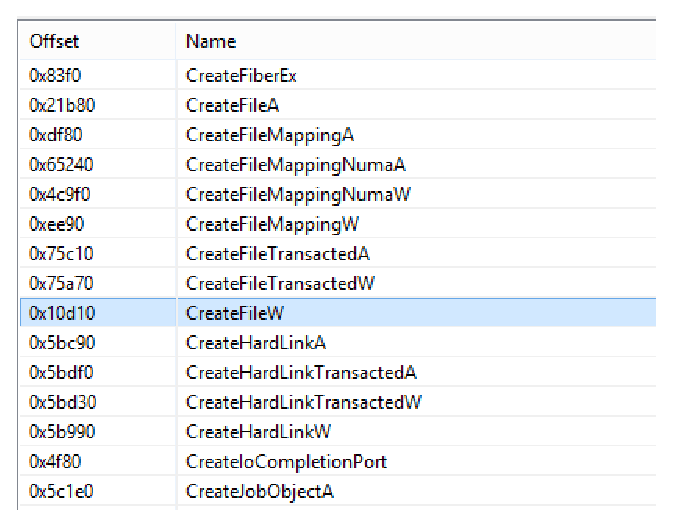
\includegraphics[scale=0.6]{Figures/executable}}
\caption{Information from kernel32.dll}
\label{executable}
\end{figure}

A new menu ``Dual\_trace Tool" with three menu options is designed for these two operations. In this menu, ``Stream Extraction" is for the operation of stream extraction and ``Communication Identification" is for the operation of communication identification. Before performing both of these two operation, The ``Load Library Exports" has to be run for both traces. ``Load Library Exports" option in this menu triggers the ``function inspect" operation for the active trace. After this operation is run separately for both traces in the dual\_trace, the traces are transformed into the proper format for communication analysis. Figure \ref{dualtracetoolmenu} shows this new menu in Atlantis. When the user performs the ``Stream Extraction" or ``Communication Identification" operations, there will be a prompt dialog window as shown in Figure \ref{methods} which asks the user what communication methods they want to analyze from the dual\_trace. This list is provided by the configuration file I mentioned in Section \ref{functionset}. The user can select one or multiple methods. Atlantis will perform the operations after the user selects and confirms the communication methods.

\begin{figure}[H]
\centerline{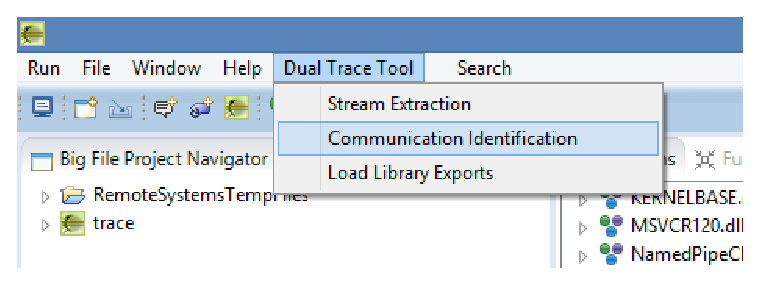
\includegraphics{Figures/dualtracetoolmenu}}
 \caption{Dual\_trace tool menu}
\label{dualtracetoolmenu}
\end{figure}

\begin{figure}[H]
\centerline{\includegraphics[scale=0.8]{Figures/methods}}
 \caption{Prompt dialog for communication selection}
\label{methods}
\end{figure}


\section{View of Extracted Streams and Identified Communications}
I designed a new view named ``Communication View" for presenting the result of the extracted streams and the identified communications. Since the user might have selected multiple selection for communication methods of interest, the output results contain all the streams or communications of all selected communication methods and the results are clustered by methods. There are two sub tables in this view, the left one is for presenting the extracted streams while the left one is for presenting identified communications. The reason for putting these two results in the same view is for easy access to and comparison of the data for the users. Figure \ref{idenview} shows this view with both extracted stream results and identified communication results in it. Each time when the user reruns the operations the result in the corresponding table will be refreshed to show only the latest result of that operation. But the other table will not be affected. For example, if the user runs the ``Stream Extraction" operation first, the extracted streams will be shown on the left table of the view. And then if the user performs the ``communication Identification" operation, the identified communications result will be shown on the right table, while the left one still holds the last stream extraction result.

\begin{figure}[H]
\centerline{\includegraphics[scale=0.7]{Figures/idenview}}
 \caption{Communication view for results}
\label{idenview}
\end{figure}

Atlantis is an analysis environment that has various views to provide user access to different information from a trace, such as the memory and register state of the current instruction line. Moreover, these views synchronize automatically with the trace view. This functionality and information also benefits the communication analysis of the dual\_trace. Providing the user a way to navigate from the result of the extracted streams and the identified communications to the trace view allows them to take advantage of the current existing functionality of Atlantis and make their analysis of the dual\_trace more efficient.

The results presented in the Communication view contains all the function call events. The memory state at the instruction line of the function begin contains the input parameters and the memory state at the instruction line of the function return contains the output parameters and the return value. In order to provide the user a method to easily access these two instruction lines, from the event entries, this implementation provides two different ways for the user to navigate back to where the function begins and ends. When the user ``double clicks" on an entry, it will bring the user to the start line of the function in the corresponding trace view. When the user right clicks on the event entry, a prompted menu with the option ``Go To Line of Function End" will show up as shown in Figure \ref{gotoend}. Clicking on this option will bring the user to the return line of this function in the trace view. All other opened views of Atlantis update immediately with this navigation. By these navigations, the users can easily see the sent and received message of the events.

\begin{figure}[H]
\centerline{\includegraphics{Figures/gotoend}}
 \caption{Right click menu on event entry}
\label{gotoend}
\end{figure}

Moreover, the ``remove" option, as shown in Figure \ref{remove}, in the right click menu on the ``stream“ or ``communication" entries is provided for the user to remove the selected ``stream" or ``communication" entry. This provides the users the flexibility to get rid of data that they are not interested about.

\begin{figure}[H]
\centerline{\includegraphics[scale=0.7]{Figures/remove}}
 \caption{Right click menu on event entry}
\label{remove}
\end{figure}

